
In Geometron we view symbols as being any geometry with meaning, including physical constructions and sequences of actions.  A ``printer'' refers to any machine which prints a symbol in this generalized sense.  This means printer now refers to a huge class of machines, really any machine with automation can be thought of as a generalized printer of symbols.  When we create symbols with the Geometron language, using the Geometron Hypercube and the Geometron Virtual Machine, we are building sequences of geometric actions, which can call other actions to build up complex fractal constructions.  One of the kinds of actions we can build into this are discrete movements of machines, just as we use discrete movements of a virtual machine when the cursor moves around on the screen building two dimensional graphics in a web browser.

\begin{figure}
	\centering
	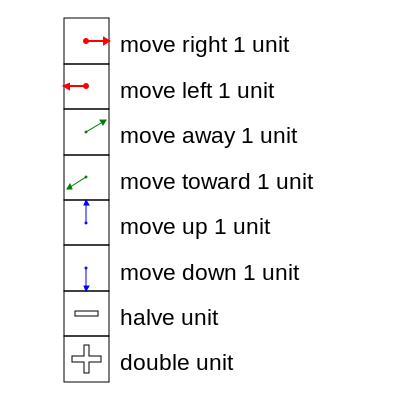
\includegraphics[width=3in]{figures/machines/basicmovements.png}
	\caption[basicmovements]
	{Basic geometric actions of machine control for an arbitrary machine that moves along three perpendicular axes.}
\end{figure}

To build up control of machines for printers, we start with the most basic discrete movements.  To begin with, we discuss the control of machines that have three axes of motion, all of which are perpendicular, along the up, down, left, right, forward, and back directions.  We start with eight basic actions: a single step in each of the six directions, doubling the step size and halving the step size.  Just these eight actions are enough to position a machine with three axis in any location in the available space.  Just as binary numbers can be used to express any decimal number, this binary approach to geometry can be used to express any geometric location.  Also note that these actions are independent of scale, and have no numerical units.  A sequence of actions is all relative to some unspecified starting unit. So a glyph created to on some agricultural tool at the 100 meter scale can print at the nanometer scale using an atomic probe of some kind with no modification to the glyph in principle.  Our language is both independent of numbers and of what machine is carrying out the actions.   

\begin{figure}
	\centering
	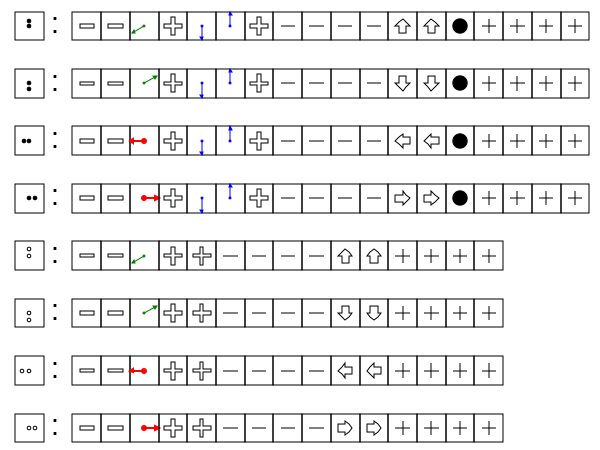
\includegraphics[width=3in]{figures/machines/actions05xx.png}
	\caption[actions05xx]
	{Dot actions from which symbols are constructed.}
\end{figure}

\begin{figure}
	\centering
	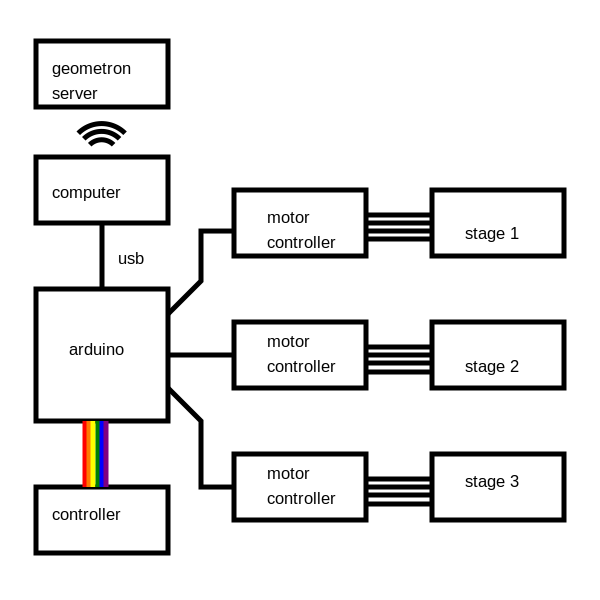
\includegraphics[width=4in]{figures/machines/printerblockdiagram.png}
	\caption[printerblockdiagram]
	{Block diagram of Trash Robot printer.  The motion stages are salvaged from DVD or CD ROM drives.  The motor drivers are off the shelf from Pololu Robotics.  The Arduino is the Arduino UNO, and the whole system including the motors gets power from the USB connected to a computer.  The computer can be used to interact with a Geoemtron server over the local network or on the global Internet to create programs which are copy/pasted into the Arduino IDE as described in the Trash Robot chapter.}
\end{figure}

\begin{figure}
	\centering
	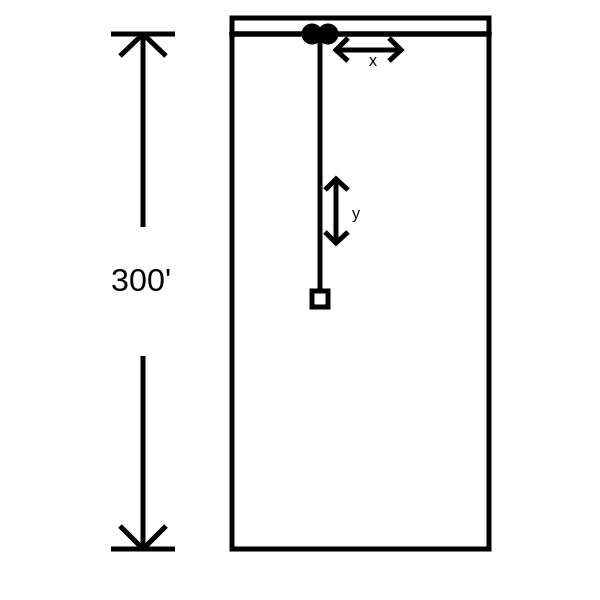
\includegraphics[width=4in]{figures/machines/buildingwallrobot.png}
	\caption[buildingwallrobot]
	{A hoist run along a rail going across the edge of a roof of a building can make a simple robot which can move to anywhere along the wall.}
\end{figure}

\begin{figure}
	\centering
	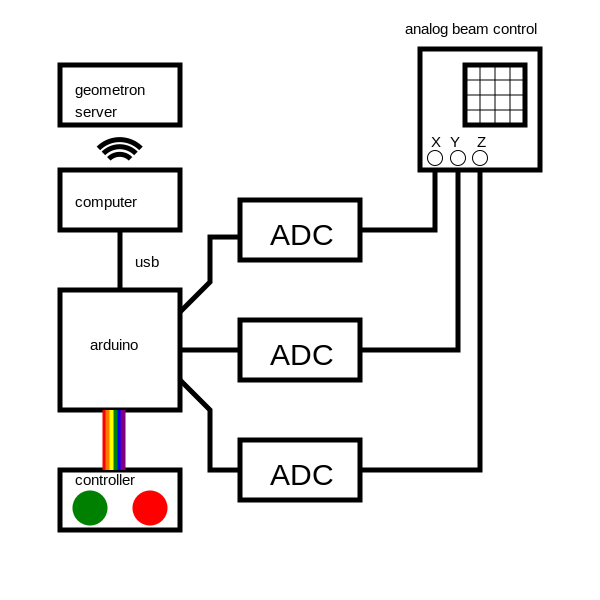
\includegraphics[width=4in]{figures/machines/eblblockdiagram.png}
	\caption[eblblockdiagram]
	{Block diagram of electron beam lithography Geometron robot.  The Arduino here drives three analog to digital converters.  Again the user can design a program for the beam path in a web browser using any computer, which can then also control and power the Arduino and its accessories.  In this case the controller only needs one huge green go button and one huge red stop button.}
\end{figure}

Icons

The idea of the icon, of a projection of it into the Geometron Hypercube and GVM.

Figure out what you want to do: what do you want to replicate from trash?  Use the idea of self-replicating set theory to make sets.  Represent the sets with icons.  Find the icons, put them in image feeds.  Trace them.  Share them.  Use them in printers.  

 printer replication

printing a print.  using it to print a stamp.  using stamps to print tokens and pendants.  Pendants are jewelry threaded onto Trash Ties throughout the system.  Tokens are used in a table top game scheme to represent sets which are used to replicate things from trash.  These are carried in water bags, along with the fire and earth bags.  Use AG to construct Sigil Boards for using the Icon Tokens on.

 bags

3d printing

laser cut spray stencil 

 earth, air, water, fire, aether